\chapter{METODOLOGIA}
\label{cap:cap02}

Neste t\'{o}pico deve ser descrito minuciosamente toda a\c{c}\~{a}o desenvolvida na aplica\c{c}\~{a}o do m\'{e}todo cient\'{\i}fico utilizado, bem como o tipo de pesquisa, instrumentos, tempo de execu\c{c}\~{a}o.
Al\'{e}m dos outros tipos de pesquisa que o trabalho pode conter, a pesquisa bibliogr\'{a}fica \'{e} uma etapa fundamental pois fornece o embasamento do trabalho. Consiste no levantamento, sele\c{c}\~{a}o, fichamento de informa\c{c}\~{o}es relacionadas \`{a} pesquisa bibliogr\'{a}fica como livros, revistas, jornais, teses, disserta\c{c}\~{o}es, anais, etc e descreve as bases de dados pesquisadas, os assuntos/ descritores/metadados, limitadores/filtros, etc. Tal etapa pode ser melhor aproveitada solicitando ajuda \`{a} Biblioteca.
\cite{Cover2006,Feynman1998,Haykin2001}

\section{Exemplo de Se\c{c}\~{a}o}
\label{sec:sec02}

Nunc malesuada posuere felis vel dapibus. Aliquam at fermentum lacus, vel malesuada elit. Duis varius nisi eget elit sagittis suscipit. Cras eu arcu at quam tristique facilisis eget vel ante. Quisque vitae libero lacinia, pellentesque tellus in, semper ligula. Aenean pharetra, elit vitae tristique pellentesque, justo erat luctus lectus, eget accumsan eros nisl vitae arcu. Proin consequat accumsan enim et porta. Aenean pharetra nulla risus, vitae ullamcorper ligula molestie in.

Integer ut elit lacus. Nullam id ullamcorper metus, et tincidunt mi. Donec blandit, sapien sit amet ultricies pharetra, turpis elit mollis risus, et pulvinar risus magna sed nunc. Sed eget risus ac risus consequat congue et ac nunc. Aenean a eros magna. Sed vel ante id ante venenatis feugiat. Sed et tortor dictum, pulvinar erat et, tempus felis. Donec pretium sagittis augue, non lacinia felis luctus a.

\begin{equation}
H(X) =-K\sum_{x\in\mathcal{X}} p_X(x)\log p_X(x),
\label{eq:shannonEntropy}
\end{equation}

A equa\c{c}\~{a}o pode ser citada assim~\eqref{eq:shannonEntropy}, e a se\c{c}\~{a}o assim~\ref{sec:sec02}

Aenean mauris sem, vulputate vitae vulputate vel, imperdiet volutpat erat. Nam malesuada pellentesque orci ac blandit. Maecenas pulvinar augue ac metus porttitor, eget tristique nunc vulputate. Sed nec mi mi. Curabitur ultrices facilisis consectetur. Cras vel urna porttitor, porta quam a, facilisis libero. Cras volutpat diam in tempor iaculis. Quisque rutrum vestibulum elit, sit amet gravida quam elementum ac. Fusce pretium hendrerit libero sed luctus. Phasellus sodales tristique purus non bibendum. Aenean faucibus pulvinar ligula, ut aliquam eros varius adipiscing. Ut a ipsum tempor, placerat quam non, imperdiet mi.

Etiam id lobortis felis, dignissim commodo est. Nunc varius nulla et aliquam venenatis. Duis non neque ut tortor gravida viverra ut nec eros. Vestibulum et felis feugiat, lacinia ante et, tempus sem. Sed quis augue varius, sagittis lacus et, scelerisque felis. Morbi nec ligula ante. Maecenas vel sodales urna, vitae accumsan nisi. Maecenas lacinia adipiscing quam, eget elementum purus feugiat at. Fusce eget dictum sem. Maecenas ante ligula, tempus non mattis quis, ultrices vel elit. Nam porta est sit amet euismod pharetra. Integer vestibulum sem a sem volutpat, vitae adipiscing massa consequat. Aliquam iaculis mi in ultrices aliquet. Donec vitae semper sapien. Vivamus vel pretium enim.

Vestibulum ante ipsum primis in faucibus orci luctus et ultrices posuere cubilia Curae; Praesent porta ligula ipsum, ac lacinia leo malesuada ac. Morbi convallis in sapien at accumsan. Nunc sit amet tempus leo, adipiscing molestie leo. Sed ut arcu consequat lacus sagittis facilisis nec sit amet diam. Fusce a gravida dolor, eu sodales tellus. Ut porta nec velit at lacinia. Mauris felis arcu, faucibus eu porta vitae, luctus a nisl. Aenean tempus felis risus, sed vehicula ante fringilla quis. Integer eget purus a diam ultricies placerat. Donec consectetur vel urna id faucibus. In accumsan iaculis imperdiet. Nam venenatis enim quis nisl mattis, quis mattis neque tincidunt. Nullam sem enim, euismod ac nisi vel, viverra imperdiet augue.

\subsection{Subse\c{c}\~{a}o}
\label{sec:subsec02}

Maecenas condimentum nunc a tincidunt fermentum. Donec lobortis fermentum ante at hendrerit. Duis et gravida nisl. Nulla auctor dui sit amet mi tempor pretium eget fermentum nisi. Nam pharetra dolor eget ipsum consectetur porta. Ut ullamcorper enim a lacus dapibus, vel malesuada tellus posuere. Suspendisse sapien enim, cursus quis bibendum cursus, dapibus vel neque. Aliquam viverra, nulla in dictum dignissim, est nulla dapibus magna, id pretium tellus orci eget lacus. Interdum et malesuada fames ac ante ipsum primis in faucibus. Ut fermentum, erat at vulputate tempus, enim lorem elementum velit, eget tempus diam arcu at leo. Proin eu neque ac erat fermentum varius nec sit amet eros. Fusce arcu mi, consequat non nibh vel, tempus bibendum orci. Nulla vel nulla massa. Nullam sit amet velit aliquet, fringilla augue ac, congue nulla. Sed dignissim, magna eu posuere luctus, libero elit posuere sem, eu euismod ligula elit non sem.

\subsection{Exemplo de Imagens}

As Figuras \ref{fig:figura_1_exemplo}, \ref{fig:figura_2_exemplo} e \ref{fig:figura_3_exemplo} ilustram como posicionar tr\^{e}s imagens em duas colunas. As Figuras \ref{fig:figura_4_exemplo}, \ref{fig:figura_5_exemplo}, \ref{fig:figura_6_exemplo}, \ref{fig:figura_7_exemplo} ilustram como posicionar 4 imagens em duas colunas e duas linhas, cada imagem com sua respectiva legenda, e como referenciar cada imagem individualmente. H\'{a} op\c{c}\~{a}o tamb\'{e}m de referenciar a imagem \ref{fig:exemplo_imagens} como um todo.

\begin{figure}[ht!]
	\centering
	\begin{minipage}[b]{.45\textwidth}
		\centering
        \subfloat[Figura 1.\label{fig:figura_1_exemplo}]{\includegraphics[width=\textwidth]{./Figuras/feec.eps}}		
	\end{minipage}\qquad
	\begin{minipage}[b]{.45\textwidth}
		\centering
		\subfloat[Figura 2.\label{fig:figura_2_exemplo}]{
\includegraphics[scale=0.2]{./Figuras/unicamp2.eps}}
		\vspace{2ex}		
		
        \subfloat[Figura 3.\label{fig:figura_3_exemplo}]{
\includegraphics[scale=1]{./Figuras/unicamp4.png}}% Note como a qualidade da imagem eps no pdf \'{e} superior visualmente
	\end{minipage}
	\caption{Exemplo de imagens.\label{fig:figuras_exemplos}}
\end{figure}

\begin{figure}
    \centering
    \subfloat[Legenda da Figura da Esquerda.\label{fig:figura_1_exemplo1}]{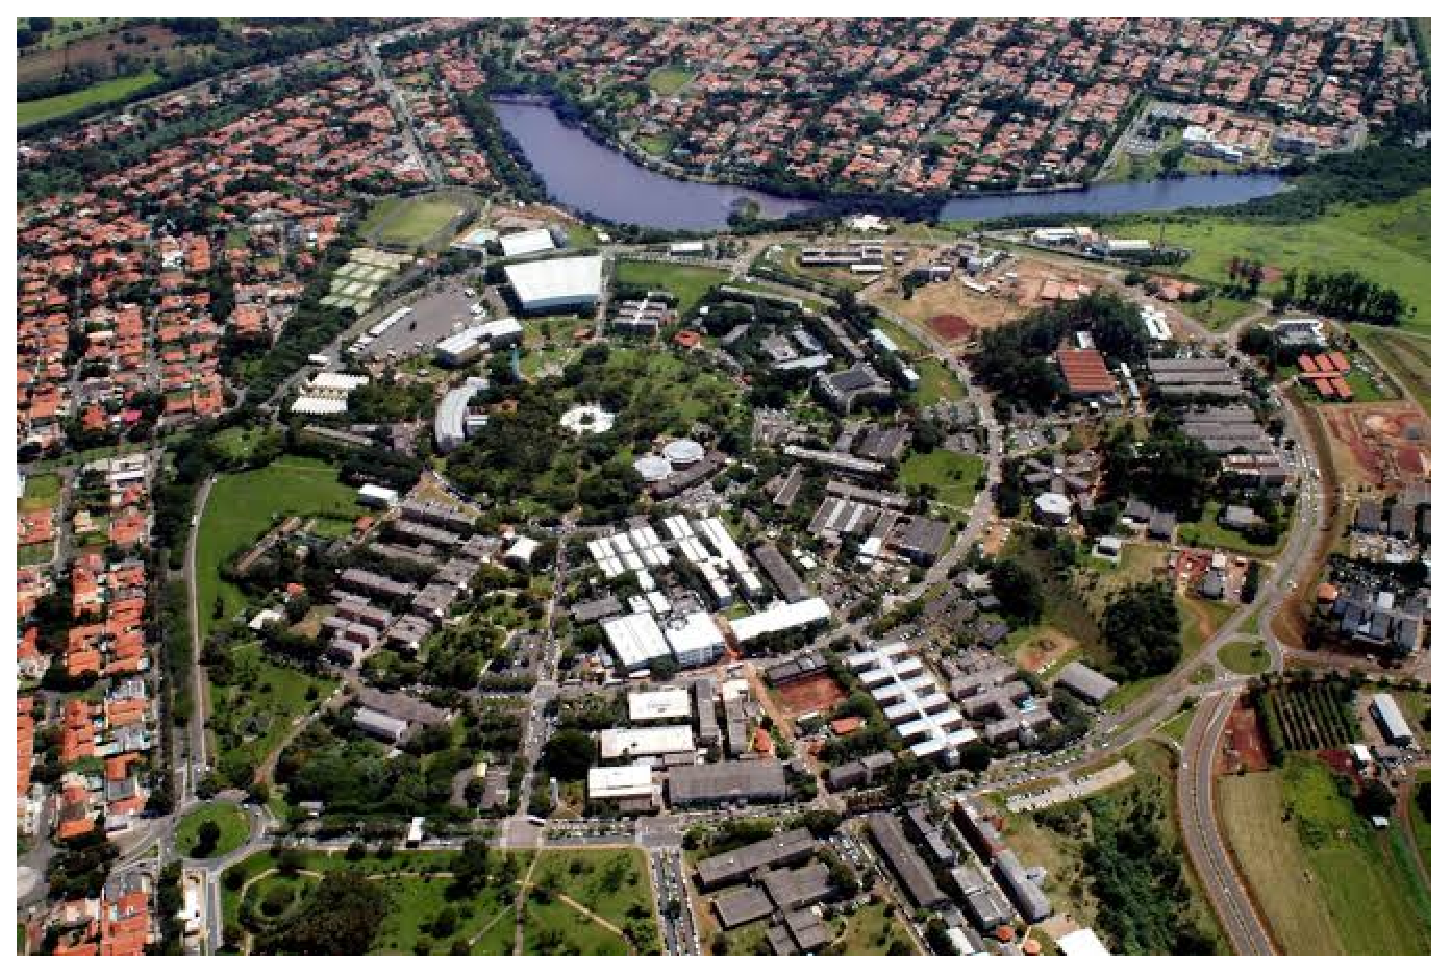
\includegraphics[width=0.40\textwidth]{./Figuras/unicamp1.eps}}
    \hspace{0.5cm}
    \subfloat[Legenda da Figura da Direita.\label{fig:figura_2_exemplo1}]{
\includegraphics[width=0.40\textwidth]{./Figuras/unicamp2.eps}}
    \caption{Figura com duas subfiguras utilizando o pacote \textit{\textbackslash subfig}}\label{fig:exemplo_2_imagens_subfloat}
\end{figure}

\begin{figure}[ht]
    \centering
    \label{ fig8}
    \begin{minipage}[b]{0.45\textwidth}
        \centering
        \subfloat[Legenda da Figura da Esquerda Superior.\label{fig:figura_4_exemplo}]{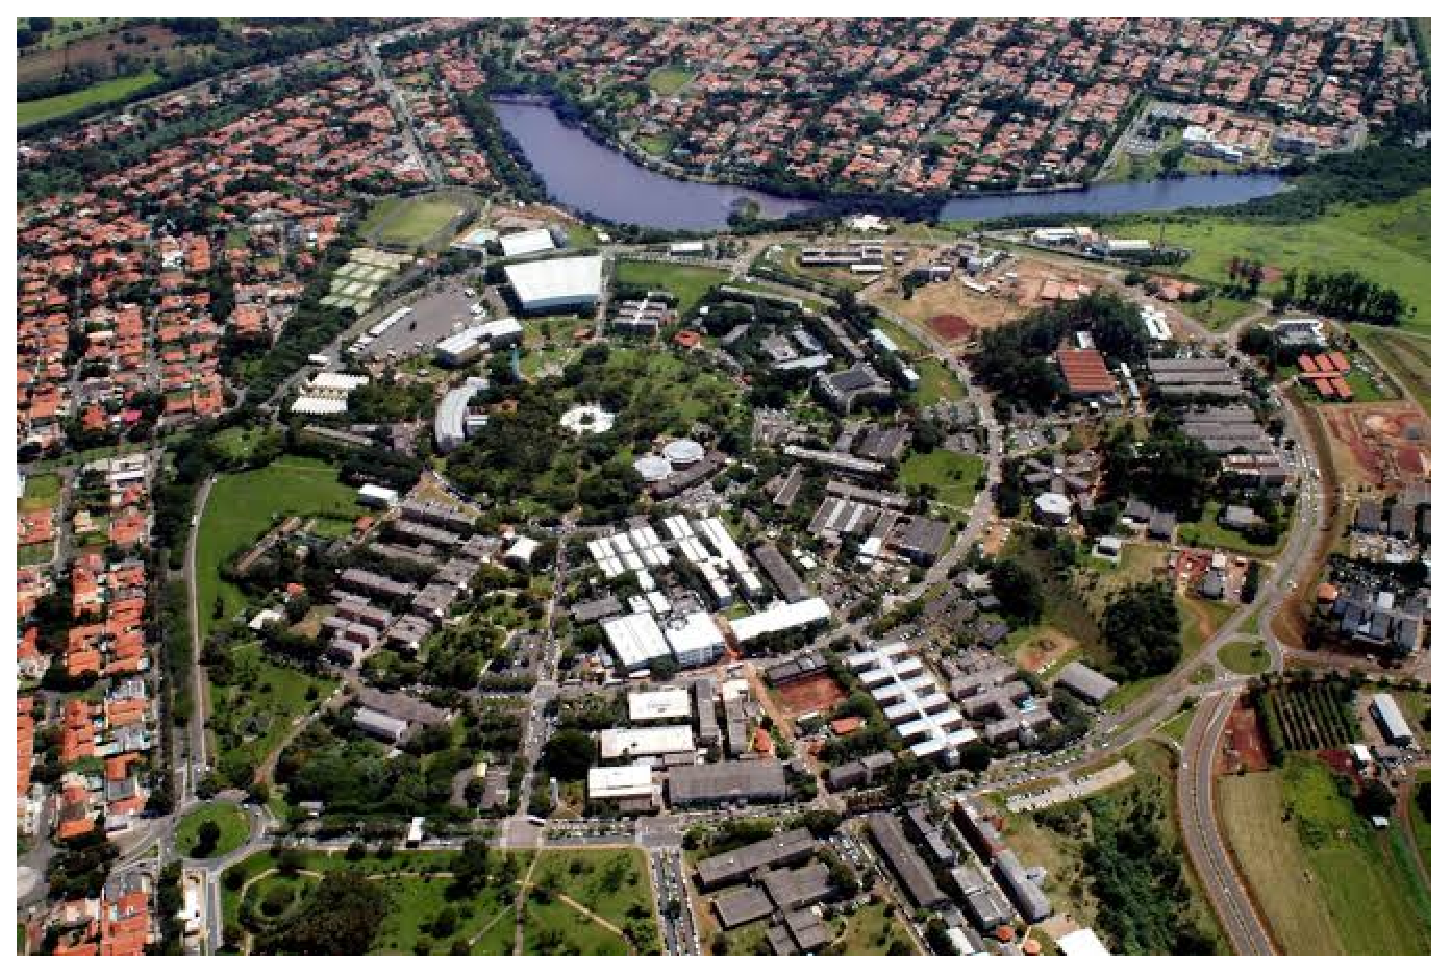
\includegraphics[width=0.9\textwidth]{./Figuras/unicamp1.eps}}
    \end{minipage}%%
    \begin{minipage}[b]{0.45\textwidth}
        \centering
        \subfloat[Legenda da Figura da Direita Superior.\label{fig:figura_5_exemplo}]{
\includegraphics[width=0.9\textwidth]{./Figuras/unicamp2.eps}}
    \end{minipage}
    \vskip\baselineskip
    \begin{minipage}[b]{0.45\textwidth}
        \centering
        \subfloat[Legenda da Figura da Esquerda Inferior.\label{fig:figura_6_exemplo}]{
\includegraphics[width=0.9\textwidth]{./Figuras/unicamp3.eps}}
    \end{minipage}%%
    \begin{minipage}[b]{0.45\textwidth}
        \centering
        \subfloat[Legenda da Figura da Direita Inferior.\label{fig:figura_7_exemplo}]{
\includegraphics[scale=1.3]{./Figuras/unicamp4.eps}}
    \end{minipage}
    \caption{Figura com quatro subfiguras utilizando o pacote \textit{\textbackslash subfig} e \textit{minipage}}\label{fig:exemplo_imagens}
\end{figure}



%\begin{figure}
%  \centering
%
%    \centering
%    \subcaptionbox{First top left}
%      {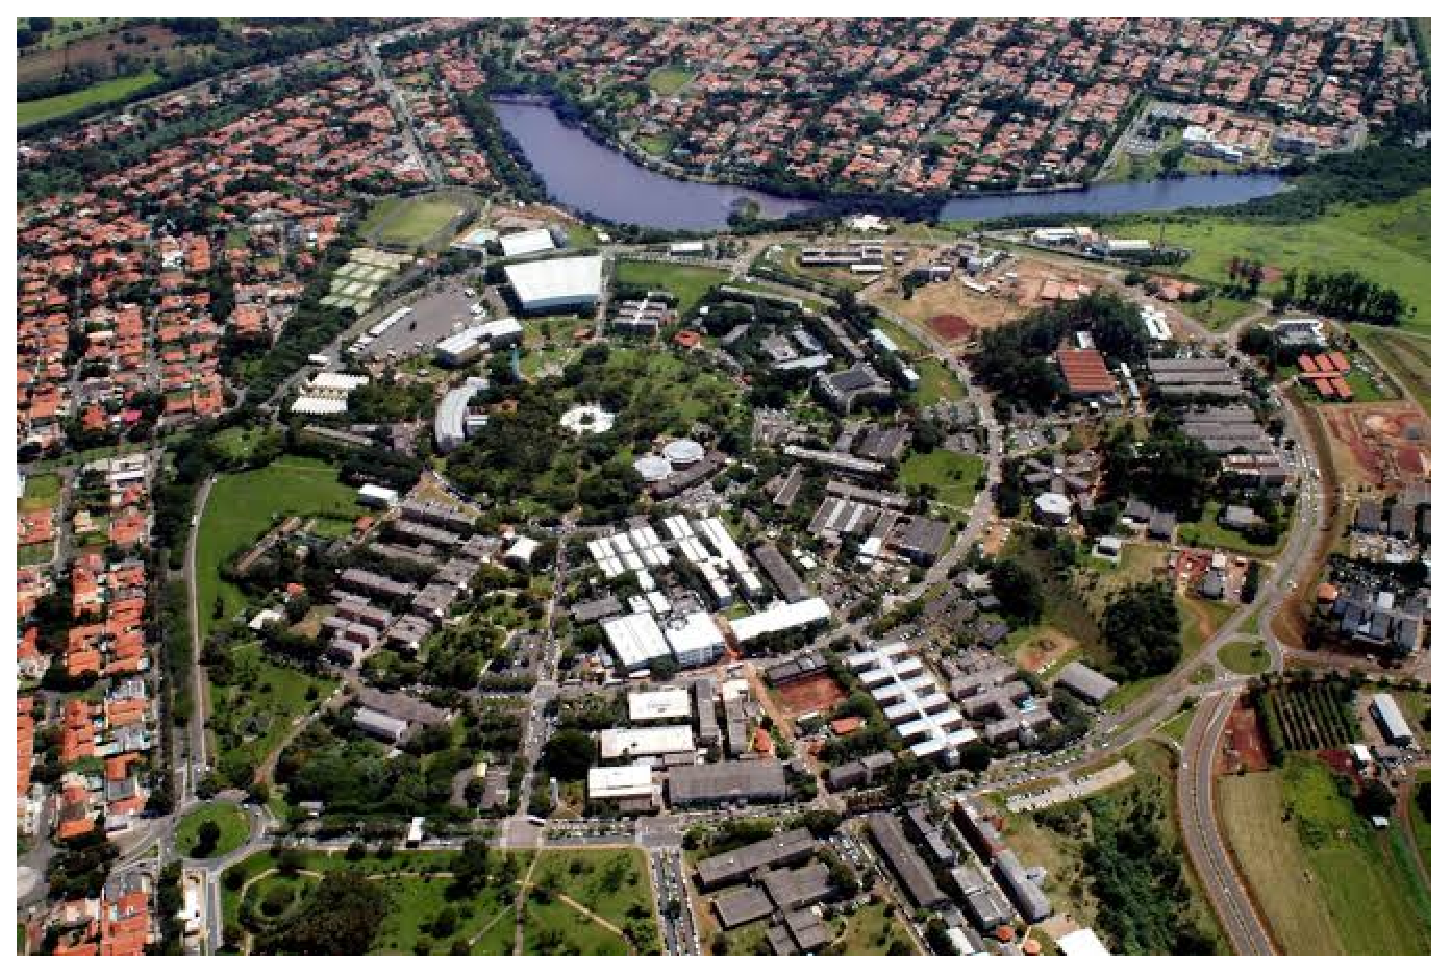
\includegraphics[width=\linewidth,height=50pt]{./Figuras/unicamp1.eps}}
%
%    \subcaptionbox{Second top left}
%      {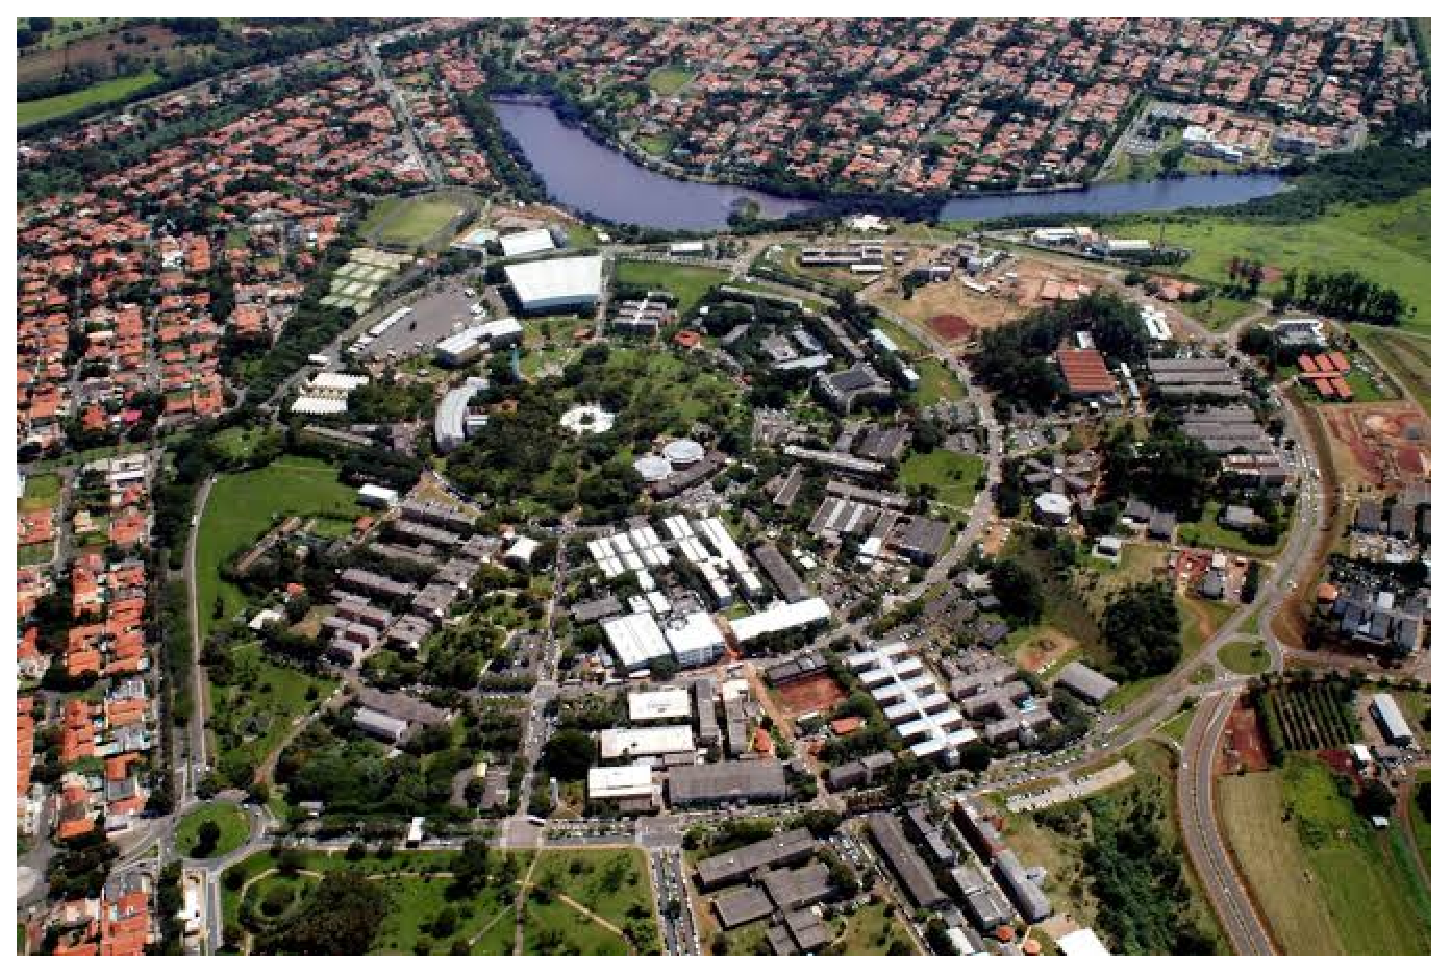
\includegraphics[width=\linewidth,height=50pt]{./Figuras/unicamp1.eps}}
%
%    \subcaptionbox{Third top left}
%      {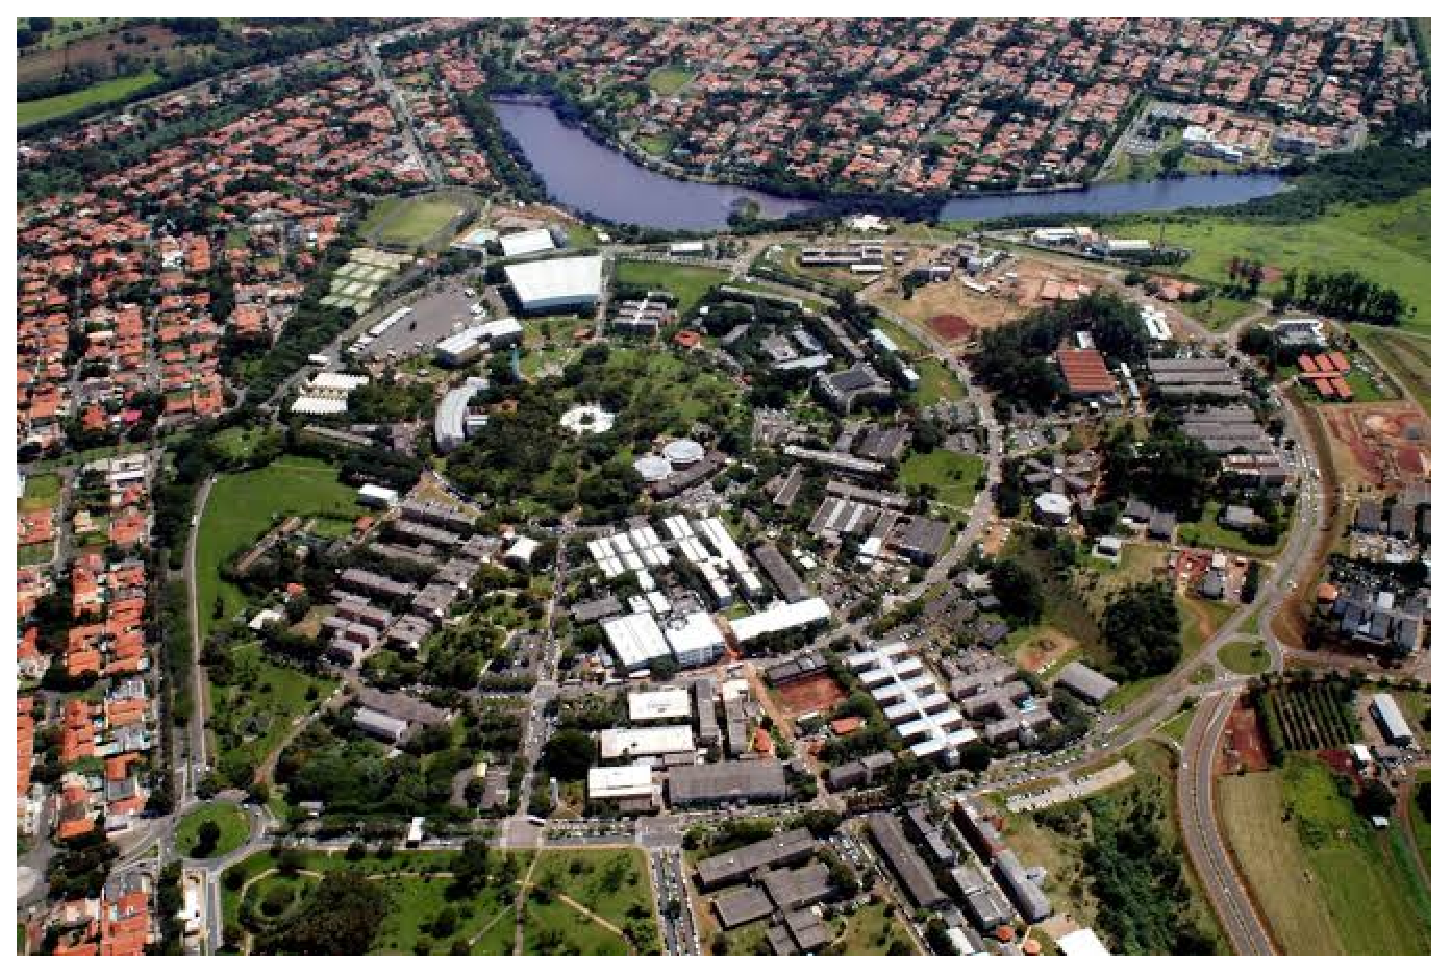
\includegraphics[width=\linewidth,height=50pt]{./Figuras/unicamp1.eps}}
%\end{figure}

%\begin{figure}[H]
%	\centering
%	\begin{subfigure}[t]{0.45\textwidth}
%		\centering
%		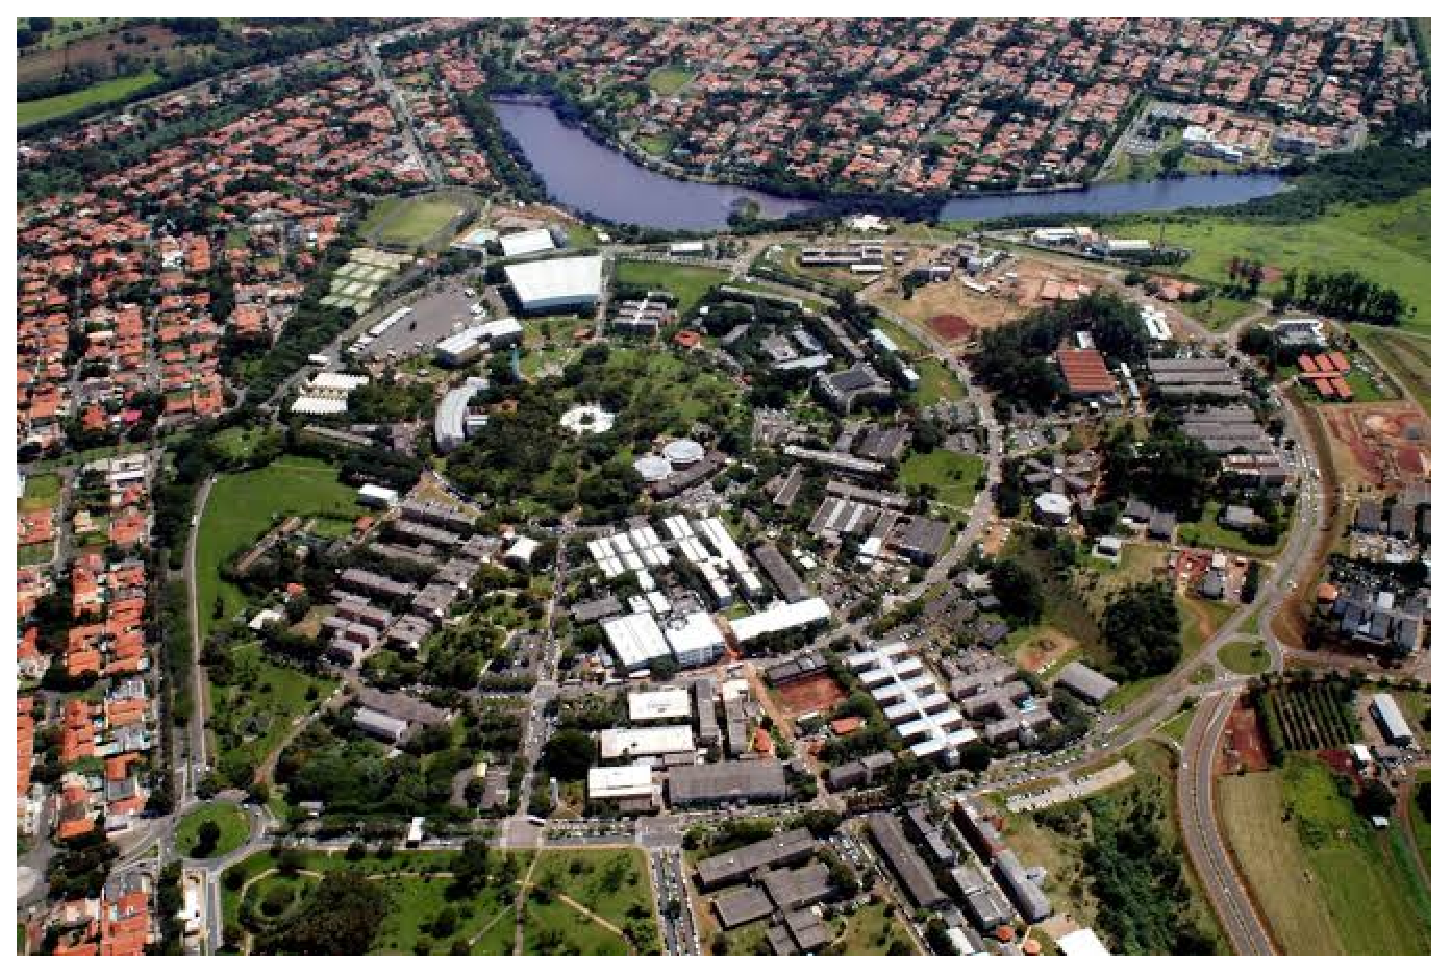
\includegraphics[width=\textwidth]{./Figuras/unicamp1.eps}
%		\caption{Figura 4.}
%		\label{fig:figura_4_exemplo}
%	\end{subfigure}%
%	~
%	\begin{subfigure}[t]{0.45\textwidth}
%		\centering
%		
\includegraphics[width=\textwidth]{./Figuras/unicamp2.eps}
%		\caption{Figura 5.}
%		\label{fig:figura_5_exemplo}
%	\end{subfigure}
%	
%	\begin{subfigure}[t]{0.45\textwidth}
%		\centering
%		
\includegraphics[width=\textwidth]{./Figuras/unicamp3.eps}
%		\caption{Figura 6.}
%		\label{fig:figura_6_exemplo}
%	\end{subfigure}%
%	~
%	\begin{subfigure}[t]{0.45\textwidth}
%		\centering
%		
\includegraphics[scale=1]{./Figuras/unicamp4.eps}
%		\caption{Figura 7.}
%		\label{fig:figura_7_exemplo}
%	\end{subfigure}
%	\caption{Exemplo de imagens.}
%	\label{fig:exemplo_imagens}
%\end{figure}
